\newpage
\section{Exercises: $Z$-transform}
\begin{enumerate}

\item Find the $z$-transforms for the following signals:
  \begin{enumerate}[a)]
  \item $h[n] = \delta[n]$
  \item $h[n] = 2\delta[n+4]$
  \item $h[n] = -41\delta[n-42]$
  \item $h[n] = \delta[n+1] - 2\delta[n-1] + 4 \delta[n-4]$
  \end{enumerate}

\item The system function $\mathcal{H}(z)$ of a discrete-time LTI system is defined as:
  \begin{equation}
    \mathcal{H}(z) = z^1 + 1 + 3z^{-1} - 0.5 z^{-2} + 4z^{-10}
    \label{eq:system_fun_eq_ex2}
  \end{equation}
  \begin{enumerate}[a)]
  \item What is the difference equation of the form:
    \begin{equation}
      y[n] = \sum_{k} \alpha_k x[n-n_k]
    \end{equation}
    that describes the relationship between the input signal $x[n]$ and the output signal $y[n]$ for the discrete-time LTI system, uniquely determined by Equation \ref{eq:system_fun_eq_ex2}?
  \item Sketch a plot of the impulse response $h[n]=\mathcal{T}\{\delta[n]\}$ of this LTI system.
  \item Modify $\mathcal{H}(z)$ in such a way that a delay by 2 samples ($y_2[n]=y[n-2]$) will be applied to the signal $y[n]$ defined in a).
  \end{enumerate}

  \begin{marginfigure}

\begin{center}
  \begin{tikzpicture}[node distance=3cm,auto,>=latex']

    \node [int] (a) {$\mathcal{H}_1(z)$};
    \node [above of=a, node distance=1cm] (in) {$x[n]$};
    \node [int, below of=a, node distance=1cm] (b) {$\mathcal{H}_1(z)$};
    \node [int, below of=b, node distance=1cm] (c) {$\mathcal{H}_1(z)$};    
    \node [below of=c, node distance=1cm] (out) {$y[n]$};
    \path[->] (a) -> (b);
    \draw[->] (a) -> (b);
    \path[->] (in) -> (a);
    \draw[->] (in) -> (a);
    \path[->] (b) -> (c);
    \draw[->] (b) -> (c);    
    \path[->] (c) -> (out);
    \draw[->] (c) -> (out);
    
    \node [int, right of=a,node distance=2cm] (a3) {$\mathcal{H}(z)$};
    \node [above of=a3, node distance=1cm] (in3) {$x[n]$};
    \node [below of=a3, node distance=1cm] (out3) {$y[n]$};
    \path[->] (in3) -> (a3);
    \draw[->] (in3) -> (a3);
    \path[->] (a3) -> (out3);
    \draw[->] (a3) -> (out3);
    
\end{tikzpicture}
\end{center}
\caption{A cascade of three elementary LTI systems defined by system functions $\mathcal{H}_1(z)$, $\mathcal{H}_2(z)$ and $\mathcal{H}_3(z)$ is equivalent to a single LTI system $\mathcal{H}(z)=\mathcal{H}_1(z)\mathcal{H}_2(z)\mathcal{H}_3(z)$.}
\label{fig:cascade_z_ex}
\end{marginfigure}

\item The system function $\mathcal{H}(z)$ of a discrete-time LTI system is defined as:
  \begin{equation}
    \mathcal{H}(z) = (z-e^{i\pi/4})(z-e^{-i\pi})z^{-2}
  \end{equation}
  You can view this system as a cascade of three elementary systems:
    \begin{equation}
      \mathcal{H}(z) = \mathcal{H}_1(z)\mathcal{H}_2(z)\mathcal{H}_3(z)
    \end{equation}
    Two of these systems will null out a single frequency and one of these systems will apply time-shift to the signal.

  \begin{enumerate}[a)]
  \item Define $\mathcal{H}_1(z)$, $\mathcal{H}_2(z)$, and $\mathcal{H}_3(z)$ and describe what each of these elementary LTI systems does to an input signal. It will be one of two options: 1) null out the frequency component with frequency $\hat{\omega}_0$, or 2) time-shift the signal by $n_0$ samples.
    
  \item Sketch the locations of the poles and zeroes of the system function on the complex plane. Include the unit circle on the plot. 
    
  \item Sketch a plot of the magnitude response $|\mathcal{H}(\hat{\omega})|$ of this system. Label the frequencies of the nulls on the horizontal axis.
  \item List the frequencies of the frequency components of the input signal that will be completely removed by this system (nulled out). Use radians per sample as the units for frequency.
  \item Write the system function in the form
    \begin{equation}
      \mathcal{H}(z) = \sum_n \alpha_n z^{-n}
    \end{equation}
    What are the non-zero values of $\alpha_n$?
  \item What is the impulse response $h[n]$ of the LTI system?
  \item If a real valued signal will be fed into the system, will the output always be real-valued? Justify your answer.
  \end{enumerate}
  
\item You have a real valued discrete-time signal that is sampled with $f_s=44.1 \cdot 10^{3}$ samples per second. Come up with a simple LTI system that will remove a 50 and 1000 hertz frequency component of the input signal. This means that the magnitude response of the LTI needs to have a null at frequencies -50, 50, -1000 and 1000 hertz. Use a suitably selected system function (z-transform of the impulse response) to derive this filter\sidenote{Remember that you can relate frequency in units of radians per sample to radians per second using $\hat{\omega}=\omega T_s$, where $T_s=1/f_s$. Also remember that you can relate frequency in units of radians per second to frequency in cycles per second (hertz) using $\omega = 2\pi f$}.

\begin{marginfigure}
\begin{center}
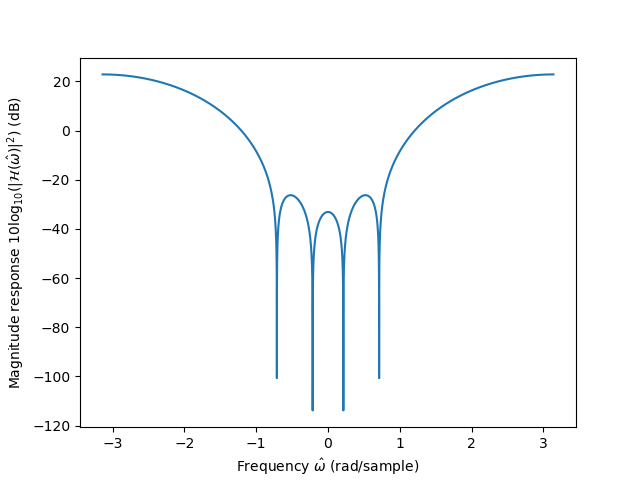
\includegraphics[width=\textwidth]{ch18/figures/ex_magresp.png}
\end{center}
\caption{Magnitude response of a filter that notches out two frequencies.}
\label{fig:2notch}
\end{marginfigure}

  \begin{enumerate}[a)] \item What is the system function that you
  came up with?  \item Draw a pole-zero diagram of your system
  function.  \item Sketch a plot of the magnitude response
  $\mathcal{H}(\hat{\omega})$ of this system.  \item Write a computer
  program to verify that the magnitude response has nulls on the
  correct frequencies. Hint: you can use the code in
  Listing \ref{lst:mag_resp_example_code} to help you out. An example
  output of this program is shown in Figure \ref{fig:2notch}.  \item
  What is the impulse response of $h[n]$ of your LTI
  system?  \end{enumerate}

  \end{enumerate}

\lstinputlisting[language=Python,caption={\texttt{030\_z\_fir\_magresp/plot\_mag\_resp.py}},label=lst:mag_resp_example_code]{code/030_z_fir_magresp/plot_mag_resp.py}